
\section{Proposed Methodology}
\subsection{Feature-space design}
For every pixel, the program builds a feature vector from one or more feature groups. Each feature channel is normalized before clustering so that one scale, such as spatial coordinate or Lab intensity, does not dominate the distance function. The tested feature groups are:
\begin{itemize}
    \item \textbf{XY:} normalized horizontal and vertical pixel positions;
    \item \textbf{RGB:} raw color channels in the standard red, green, and blue representation;
    \item \textbf{HSV:} hue, saturation, and value channels for illumination-aware color separation;
    \item \textbf{Lab:} perceptually motivated lightness and chromaticity channels;
    \item \textbf{Texture:} local texture responses using Gabor, Leung--Malik, or GLCM-style descriptors depending on the image group;
    \item \textbf{Combinations:} XY + color, XY + texture, color + texture, and XY + color + texture.
\end{itemize}

The idea is that color separates regions with different appearance, XY penalizes spatially scattered clusters, and texture separates regions with similar color but different surface pattern. This is especially useful for natural images where object boundaries are often defined by texture changes rather than color alone.

\subsection{Texture features}
Gabor filters are useful for orientation- and frequency-selective texture analysis. In this implementation a multi-scale, multi-orientation bank is applied to the grayscale image and the absolute filter responses are used as texture channels. For images where material-like texture is more important, a Leung--Malik-style bank of Gaussian derivatives and isotropic filters is used. For some images, GLCM-style texture outputs are included in the generated results, especially where co-occurrence statistics were more stable than direct filter responses.

\begin{figure}[H]
\centering
\begin{subfigure}{0.47\textwidth}
\centering
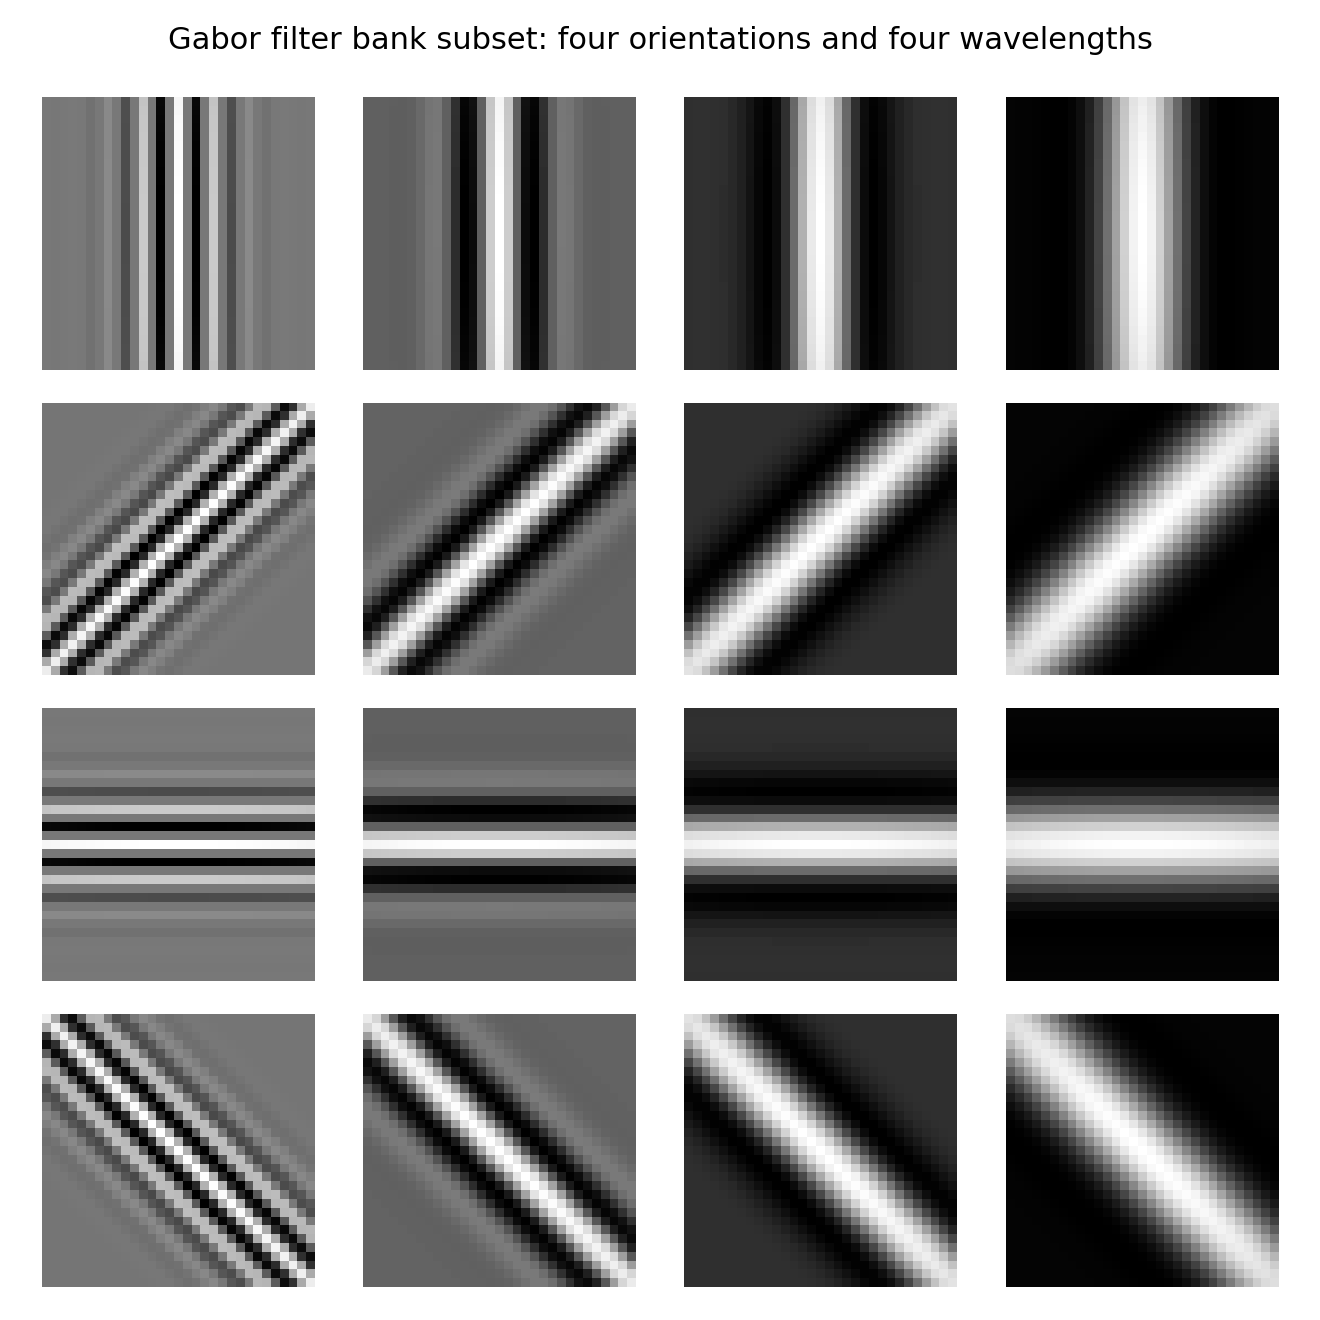
\includegraphics[width=\textwidth]{figures/method/gabor_filter_bank_subset.png}
\caption{Subset of the Gabor bank.}
\end{subfigure}\hfill
\begin{subfigure}{0.47\textwidth}
\centering
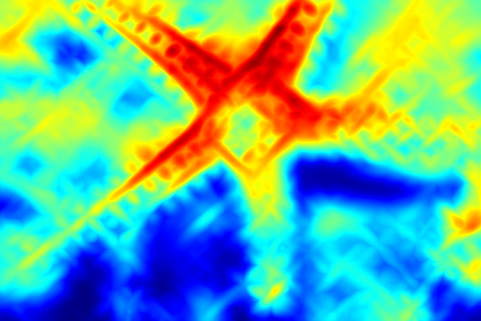
\includegraphics[width=\textwidth]{figures/method/gabor_activation_img01.png}
\caption{JET heat map of maximum Gabor response on Image 01.}
\end{subfigure}
\caption{Gabor filter visualization and response map. The heat map highlights pixels where at least one filter in the bank activates strongly.}
\label{fig:gabor-method}
\end{figure}

\begin{figure}[H]
\centering
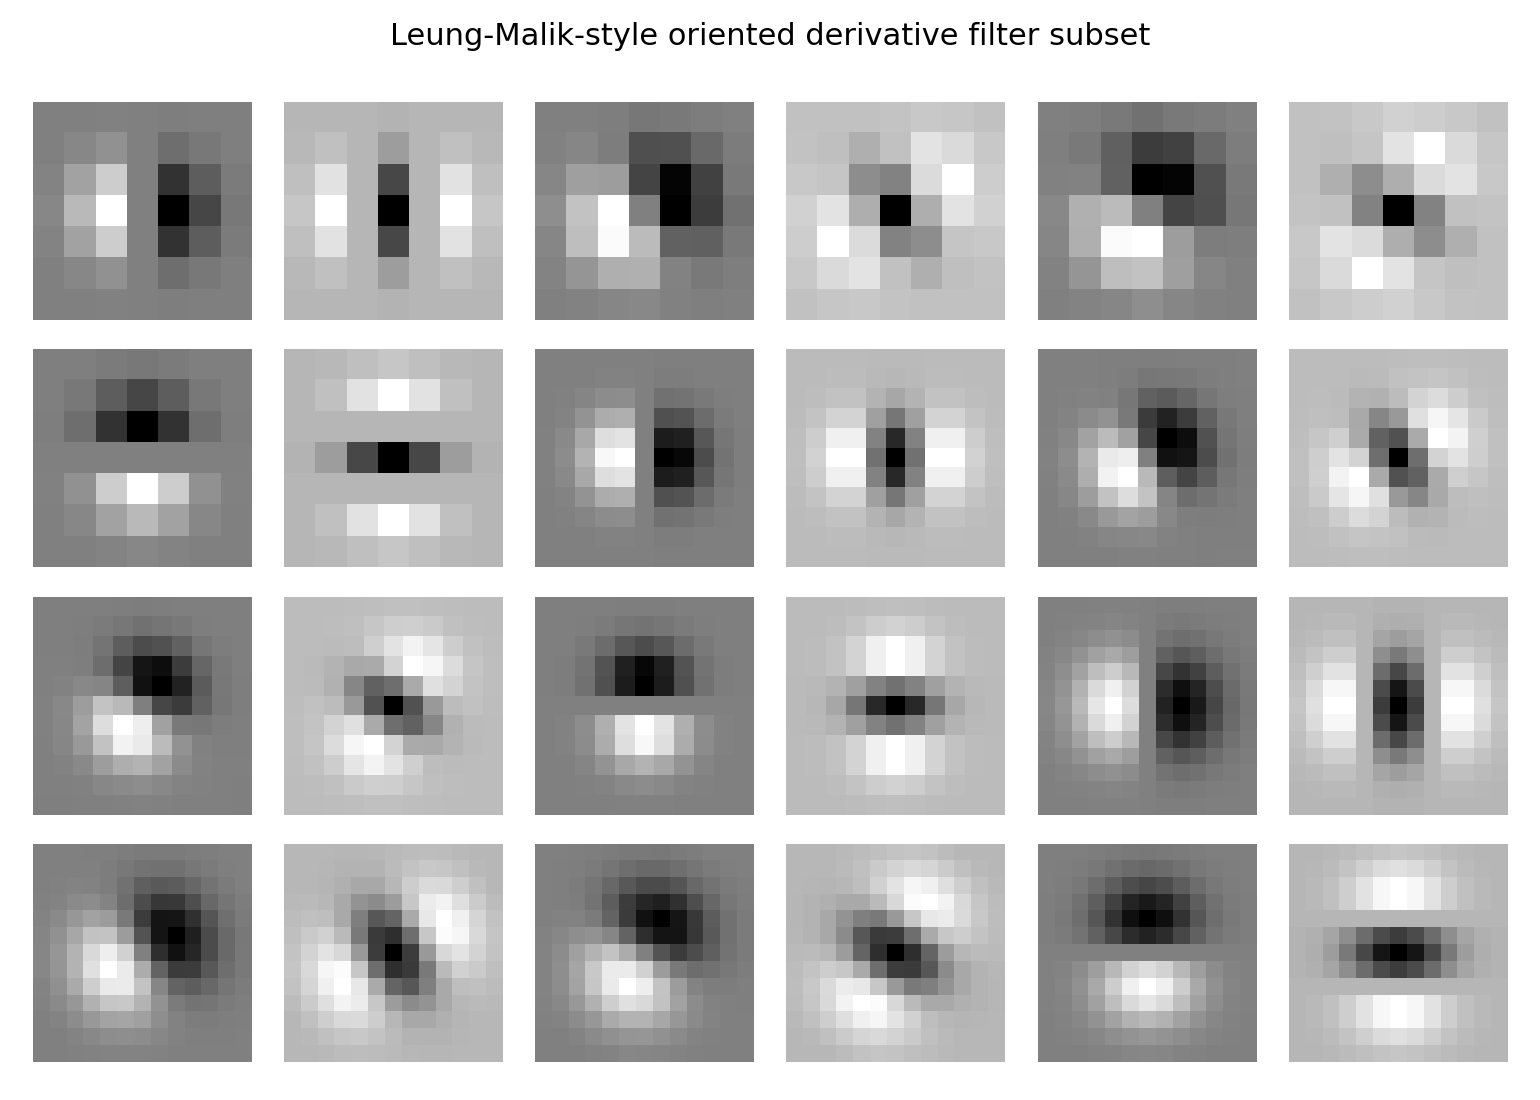
\includegraphics[width=0.72\textwidth]{figures/method/lm_filter_bank_subset.png}
\caption{Representative subset of the Leung--Malik-style oriented derivative filter bank used for texture representation.}
\label{fig:lm-method}
\end{figure}

\subsection{Clustering algorithms}
Two unsupervised clustering strategies are used.
\textbf{MiniBatch K-means} is used as the fast fixed-cluster baseline. It uses K-means++ initialization and mini-batches to reduce computation time. Most runs use $K=5$, while additional $K=4$ and $K=10$ outputs are stored for selected images to study under- and over-segmentation.

\textbf{Mean Shift} is used as an adaptive mode-seeking method. Two bandwidth values are tested in most output batches. Because Mean Shift becomes expensive in high-dimensional spaces, the implementation includes three practical modes: sampled Mean Shift, quarter-size Mean Shift, and half-size Mean Shift with PCA retaining 95\% variance. This directly follows the assignment note that resizing and PCA may be used to make Mean Shift feasible.

\subsection{Post-processing}
After clustering, small connected components are removed. Each small component is assigned to the most common surrounding label in a local dilation neighborhood. This step reduces isolated fragments and makes the segmentation more region-like without changing the main cluster structure. The report and CSVs use the post-processed masks, which are the final deliverable outputs.
